\documentclass[11pt,a4paper]{article}

\usepackage[margin=2.3cm]{geometry}
\usepackage[T1]{fontenc}
\usepackage[utf8]{inputenc}
\usepackage{amsmath,amssymb,amsthm,mathtools}
\usepackage{booktabs,array,tabularx}
\usepackage{enumitem}
\usepackage{xcolor}
\usepackage{tikz}
\usetikzlibrary{arrows.meta,calc,positioning,shapes.geometric,decorations.pathreplacing,backgrounds}
\usepackage{pgfplots}
\pgfplotsset{compat=1.16}
\usepackage[most]{tcolorbox}
\usepackage[hidelinks]{hyperref}
\usepackage{caption}
\usepackage{float}
\captionsetup{font=small,labelfont=bf}

% ---------- macros ----------
\newcommand{\Ts}{T_s}
\newcommand{\hx}{\hat{\boldsymbol{x}}}
\newcommand{\hq}{\hat{\boldsymbol{q}}}
\newcommand{\bx}{\boldsymbol{x}}
\newcommand{\bq}{\boldsymbol{q}}
\newcommand{\bu}{\boldsymbol{u}}
\newcommand{\by}{\boldsymbol{y}}
\newcommand{\bv}{\boldsymbol{v}}
\newcommand{\bw}{\boldsymbol{w}}
\newcommand{\bnu}{\boldsymbol{\nu}}
\newcommand{\mA}{\mathbf{A}}
\newcommand{\mB}{\mathbf{B}}
\newcommand{\mC}{\mathbf{C}}
\newcommand{\mF}{\mathbf{F}}
\newcommand{\mH}{\mathbf{H}}
\newcommand{\mP}{\mathbf{P}}
\newcommand{\mR}{\mathbf{R}}
\newcommand{\mS}{\mathbf{S}}
\newcommand{\mV}{\mathbf{V}}
\newcommand{\mW}{\mathbf{W}}
\newcommand{\mI}{\mathbf{I}}
\newcommand{\pinv}{^{\dagger}}
\newcommand{\tp}{^{\top}}
\newcommand{\E}{\mathbb{E}}
\newcommand{\Rn}{\mathbb{R}}
\DeclareMathOperator{\atantwo}{atan2}
\DeclareMathOperator{\sinc}{sinc}
\DeclareMathOperator{\diag}{diag}
\newcommand{\slides}[1]{\texorpdfstring{\hspace{0.5em}{\normalfont\small\emph{(#1)}}}{}}

% ---------- theorem-like environments (amsthm) ----------
\theoremstyle{plain}
\newtheorem{theorem}{Theorem}[section]
\newtheorem{lemma}[theorem]{Lemma}
\newtheorem{proposition}[theorem]{Proposition}
\newtheorem{corollary}[theorem]{Corollary}
\theoremstyle{definition}
\newtheorem{definition}[theorem]{Definition}
\newtheorem{example}[theorem]{Example}
\newtheorem{algorithm}[theorem]{Algorithm}
\theoremstyle{remark}
\newtheorem*{remark}{Remark}

\tcbset{thmbox/.style={enhanced,breakable,colback=gray!5,colframe=black!55,boxrule=0.5pt,arc=2pt,
  left=6pt,right=6pt,top=4pt,bottom=4pt,before skip=10pt,after skip=10pt}}
\tcolorboxenvironment{theorem}{thmbox}
\tcolorboxenvironment{lemma}{thmbox}
\tcolorboxenvironment{proposition}{thmbox}
\tcolorboxenvironment{corollary}{thmbox}
\tcolorboxenvironment{definition}{thmbox,colback=green!4,colframe=green!40!black}
\tcolorboxenvironment{example}{thmbox,colback=orange!5,colframe=orange!65!black}
\tcolorboxenvironment{algorithm}{thmbox,colback=violet!4,colframe=violet!60!black}

\newtcolorbox{intuition}{enhanced,breakable,colback=blue!5,colframe=blue!60!black,coltitle=white,
  colbacktitle=blue!60!black,fonttitle=\bfseries,title={Intuition},boxrule=0.6pt,arc=2pt,
  left=6pt,right=6pt,top=3pt,bottom=3pt,before skip=10pt,after skip=12pt}

\newtcolorbox{placeholder}[1]{enhanced,colback=white,colframe=red!60!black,boxrule=0.8pt,
  fonttitle=\bfseries\small,coltitle=red!60!black,colbacktitle=white,
  title={IMAGE PLACEHOLDER},halign=center,valign=center,height=6.2cm,before skip=10pt,after skip=10pt}

\setlist[itemize]{itemsep=2pt,topsep=4pt}
\setlist[enumerate]{itemsep=2pt,topsep=4pt}

\title{\textbf{Autonomous and Mobile Robotics}\\[4pt]
\Large Localization: Odometric Localization and the Extended Kalman Filter}
\author{Course of Prof.\ Giuseppe Oriolo --- Sapienza Universit\`a di Roma}
\date{\today}

\begin{document}
\maketitle
\tableofcontents

\bigskip
\noindent\textbf{Conventions.} Slide ranges in the section headers refer to the \emph{Odometric
Localization} deck (Sections~1--4) or to the \emph{Extended Kalman Filter} deck (Sections~5--10).
Section~11 is the application worked out in the companion book chapter (Sect.~7.7.2 there), merged
at the point where the EKF has just been introduced. The robot is a unicycle with configuration
$\bq=(x,y,\theta)$, kinematic inputs $v$ (driving velocity) and $\omega$ (steering velocity),
and sampling interval $\Ts=t_{k+1}-t_k$.

% =====================================================================
\section{Why localization is needed \slides{odometry deck, slide 2}}
% =====================================================================

Planning and, above all, feedback control need the robot configuration $\bq$ at every time instant:
a trajectory-tracking law computes its commands from the \emph{error} between the desired and the
actual configuration, so it cannot even be written down without an estimate of $\bq$.

For a robot manipulator this is easy: joint encoders measure the joint variables, which
\emph{are} the configuration. A wheeled mobile robot (WMR) is different. Its incremental encoders
measure only how much each wheel has rotated, \emph{not} where the vehicle is with respect to a fixed
world frame.

\begin{definition}[Localization]
\emph{Localization} is a procedure that estimates, typically in real time, the configuration
$\bq(t)$ of a robot with respect to a fixed world frame from the available sensor data.
\end{definition}

\begin{intuition}
A joint encoder is like a GPS: it tells you directly \emph{where} you are. A wheel encoder is like a
pedometer: it tells you how many steps you took, from which you can \emph{reconstruct} where you are
only if you know where you started and how long and in which direction each step was. The whole
lecture follows this analogy: first we add up the steps (odometry), then we learn to correct the
sum by looking around (Kalman filtering with exteroceptive sensors).
\end{intuition}

% =====================================================================
\section{Odometric localization: integrating the kinematic model \slides{odometry deck, slides 3--6}}
% =====================================================================

\subsection{Setting: constant inputs over a sampling interval}

Recall the unicycle kinematic model
\begin{equation}\label{eq:unicycle}
\dot x = v\cos\theta,\qquad \dot y = v\sin\theta,\qquad \dot\theta=\omega .
\end{equation}
In a digital implementation the velocity inputs are held constant over each sampling interval:
$v(t)=v_k$, $\omega(t)=\omega_k$ for $t\in[t_k,t_{k+1})$. Then $\theta(t)=\theta_k+\omega_k(t-t_k)$,
so the heading changes at a constant rate, and the robot moves along an arc of circle of radius
$|v_k/\omega_k|$ (a line segment if $\omega_k=0$).

\medskip
\noindent\textbf{Problem.} Given $\bq_k=(x_k,y_k,\theta_k)$ and $(v_k,\omega_k)$, compute $\bq_{k+1}$
by integrating \eqref{eq:unicycle} over $[t_k,t_{k+1}]$.

\begin{intuition}
Constant ``gas'' and constant ``steering wheel'' means driving on a circle. Over one sampling
interval the robot therefore covers a short arc; the only question is how faithfully we want to
reproduce that arc with a formula.
\end{intuition}

\subsection{Three integration schemes}

\begin{algorithm}[Euler integration]\label{alg:euler}
\begin{align}
x_{k+1}&=x_k+v_k\Ts\cos\theta_k,\nonumber\\
y_{k+1}&=y_k+v_k\Ts\sin\theta_k,\label{eq:euler}\\
\theta_{k+1}&=\theta_k+\omega_k\Ts .\nonumber
\end{align}
$x_{k+1}$ and $y_{k+1}$ are \emph{approximate} (computed as if the orientation stayed equal to
$\theta_k$ throughout the interval); $\theta_{k+1}$ is \emph{exact}.
\end{algorithm}

\begin{algorithm}[Second-order Runge--Kutta integration]\label{alg:rk}
\begin{align}
x_{k+1}&=x_k+v_k\Ts\cos\!\Big(\theta_k+\frac{\omega_k\Ts}{2}\Big),\nonumber\\
y_{k+1}&=y_k+v_k\Ts\sin\!\Big(\theta_k+\frac{\omega_k\Ts}{2}\Big),\label{eq:rk}\\
\theta_{k+1}&=\theta_k+\omega_k\Ts .\nonumber
\end{align}
The \emph{average orientation} over $[t_k,t_{k+1}]$ is used; $x_{k+1},y_{k+1}$ are still
approximate but more accurate.
\end{algorithm}

\begin{proposition}[Exact integration]\label{prop:exact}
Under constant $v_k,\omega_k$ with $\omega_k\neq 0$,
\begin{align}
x_{k+1}&=x_k+\frac{v_k}{\omega_k}\big(\sin\theta_{k+1}-\sin\theta_k\big),\nonumber\\
y_{k+1}&=y_k-\frac{v_k}{\omega_k}\big(\cos\theta_{k+1}-\cos\theta_k\big),\label{eq:exact}\\
\theta_{k+1}&=\theta_k+\omega_k\Ts .\nonumber
\end{align}
For $\omega_k\to0$ the first two formulas tend to the Euler (and Runge--Kutta) ones, so they remain
defined at $\omega_k=0$.
\end{proposition}
\begin{proof}
Since $\theta(t)=\theta_k+\omega_k(t-t_k)$ we have $dt=d\theta/\omega_k$, hence
\[
x_{k+1}-x_k=\int_{t_k}^{t_{k+1}}v_k\cos\theta\,dt=\frac{v_k}{\omega_k}\int_{\theta_k}^{\theta_{k+1}}\cos\theta\,d\theta
=\frac{v_k}{\omega_k}(\sin\theta_{k+1}-\sin\theta_k),
\]
and similarly for $y$. For the limit, $\sin(\theta_k+\omega_k\Ts)-\sin\theta_k=\omega_k\Ts\cos\theta_k+O(\omega_k^2)$,
so $x_{k+1}-x_k\to v_k\Ts\cos\theta_k$ (and likewise for $y$) as $\omega_k\to0$.
\end{proof}

\begin{intuition}
For $\omega_k\approx0$ the exact formula is a ``$0/0$'' expression: numerically it divides a tiny
number by a tiny number. In an implementation one therefore adds a conditional instruction: if
$|\omega_k|$ is below a small threshold use the straight-line (Euler/Runge--Kutta) update, otherwise
the closed form.
\end{intuition}

\subsection{How different are they? Geometry and error order}

Figure~\ref{fig:three} compares the three reconstructions of $\bq_{k+1}$ on a single arc.

\begin{figure}[H]
	\centering
	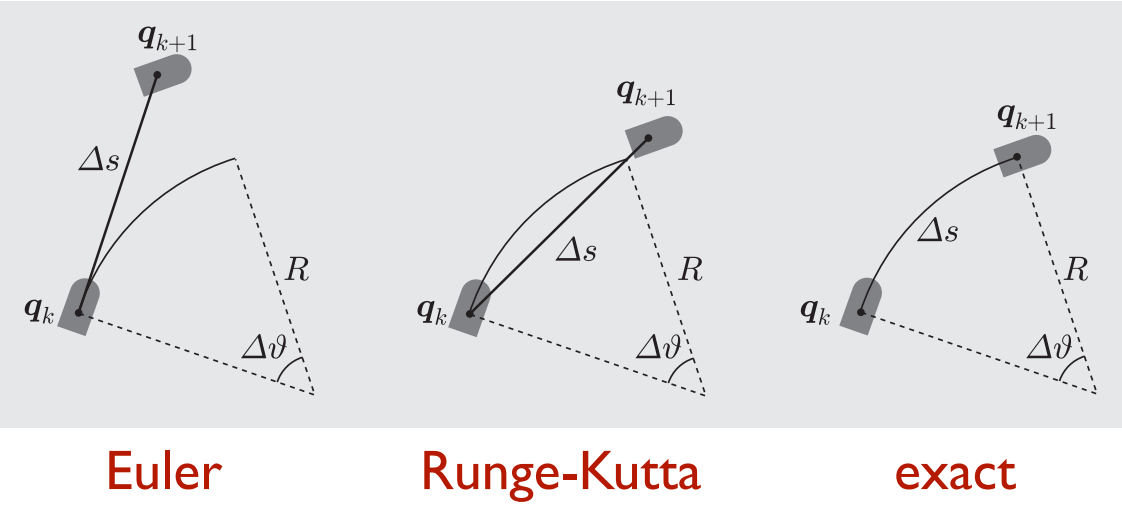
\includegraphics[width=1.0\linewidth]{1793864973959.png}
	\caption{Odometric localization of a unicycle over one arc of circle (redrawn). Euler moves along the
initial heading; Runge--Kutta moves along the \emph{mean} heading; the exact formula follows the arc.
The small grey circle marks the exact end point. The arc here is exaggerated ($\Delta\theta=60^\circ$);
at realistic sampling rates the three points almost coincide.}\label{fig:three}
\end{figure}


\begin{proposition}[Leading-order error of the schemes]\label{prop:error}
Let $a=\omega_k\Ts/2$. The exact update equals the Runge--Kutta one with the step length scaled by
$\sinc(a)=\sin a/a$:
\begin{equation}\label{eq:sinc}
\begin{aligned}
x_{k+1}-x_k&=v_k\Ts\,\sinc(a)\cos(\theta_k+a),\\
y_{k+1}-y_k&=v_k\Ts\,\sinc(a)\sin(\theta_k+a).
\end{aligned}
\end{equation}
Consequently, to leading order the position error \emph{per step} is
$\tfrac12 v_k\omega_k\Ts^2$ for Euler and $\tfrac1{24}v_k\omega_k^2\Ts^3$ for Runge--Kutta.
\end{proposition}
\begin{proof}
Use $\sin\alpha-\sin\beta=2\cos\frac{\alpha+\beta}2\sin\frac{\alpha-\beta}2$ with $\alpha=\theta_{k+1}$,
$\beta=\theta_k$:
$\frac{v_k}{\omega_k}(\sin\theta_{k+1}-\sin\theta_k)=\frac{2v_k}{\omega_k}\sin(a)\cos(\theta_k+a)=v_k\Ts\sinc(a)\cos(\theta_k+a)$.
The $y$ formula is analogous with $\cos\beta-\cos\alpha=2\sin\frac{\alpha+\beta}2\sin\frac{\alpha-\beta}2$.
Now $\sinc(a)=1-a^2/6+\dots=1-(\omega_k\Ts)^2/24+\dots$, so Runge--Kutta (which sets $\sinc=1$) errs by
about $v_k\Ts\,(\omega_k\Ts)^2/24$. Euler uses the heading $\theta_k$ instead of $\theta_k+a$: its step vector
is rotated by the angle $a$ with respect to the exact one, giving an error of about $v_k\Ts\,a=\tfrac12v_k\omega_k\Ts^2$.
\end{proof}

\begin{intuition}
Euler commits to the \emph{starting} heading, Runge--Kutta to the \emph{average} heading, and the exact
formula additionally knows that a chord is shorter than its arc (the $\sinc$ factor). Taking the heading
at the middle of the interval is what removes the dominant error: halve $\Ts$ and the Euler error per step
drops by a factor $4$, the Runge--Kutta one by a factor $8$ (Fig.~\ref{fig:rates}). This is why the
differences ``tend to disappear as the sampling rate increases''.
\end{intuition}

\begin{figure}[H]
\centering
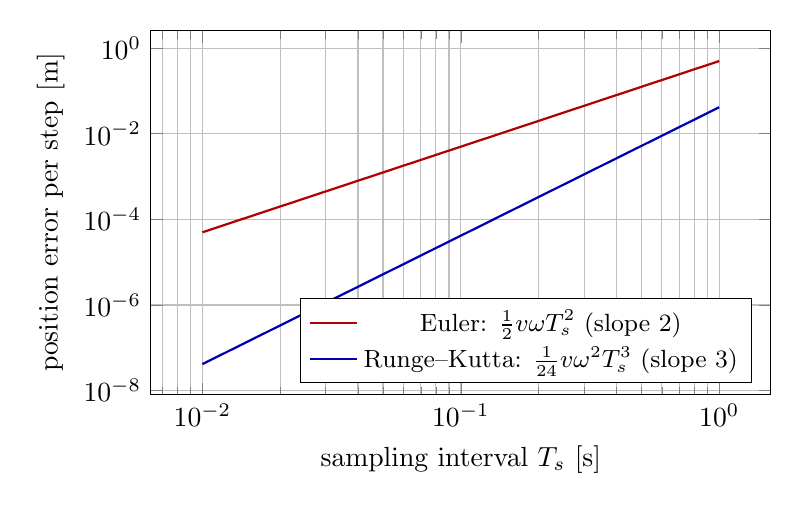
\begin{tikzpicture}
\begin{axis}[width=0.78\linewidth,height=6.2cm,xmode=log,ymode=log,grid=both,domain=0.01:1,
  xlabel={sampling interval $\Ts$ [s]},ylabel={position error per step [m]},
  legend pos=south east,legend style={font=\small},samples=20]
\addplot[red!70!black,thick] {0.5*x^2};
\addlegendentry{Euler: $\tfrac12 v\omega\Ts^2$ (slope 2)}
\addplot[blue!70!black,thick] {x^3/24};
\addlegendentry{Runge--Kutta: $\tfrac1{24}v\omega^2\Ts^3$ (slope 3)}
\end{axis}
\end{tikzpicture}
\caption{Leading-order local error of the two approximate schemes for $v=1$ m/s, $\omega=1$ rad/s
(illustrative asymptotics from Prop.~\ref{prop:error}).}\label{fig:rates}
\end{figure}

\begin{example}[A coarse step, numerically]
Take $\theta_k=0$, $v_k=1$ m/s, $\omega_k=\pi/2$ rad/s and $\Ts=1$ s (a quarter turn in one step, deliberately coarse).
\begin{center}
\begin{tabular}{lcc}
\toprule
Scheme & $(x_{k+1}-x_k,\;y_{k+1}-y_k)$ [m] & distance from exact\\
\midrule
Euler & $(1,\;0)$ & $0.733$\\
Runge--Kutta & $(0.707,\;0.707)$ & $0.100$\\
Exact & $(2/\pi,\;2/\pi)=(0.637,\;0.637)$ & $0$\\
\bottomrule
\end{tabular}
\end{center}
Check with \eqref{eq:sinc}: $a=\pi/4$, $\sinc(a)=0.900$, and $0.900\cdot0.707=0.637$.
\end{example}

% =====================================================================
\section{Reconstructing the inputs from proprioceptive sensors \slides{odometry deck, slide 7}}
% =====================================================================

The formulas above assume that $v_k,\omega_k$ are known. But no actuation system is ideal: the
\emph{commanded} inputs are not what the robot actually executes. It is therefore better to
reconstruct $v_k$ and $\omega_k$ from their \emph{effect}:
\begin{equation}\label{eq:ds}
v_k\Ts=\Delta s,\qquad \omega_k\Ts=\Delta\theta,\qquad \frac{v_k}{\omega_k}=\frac{\Delta s}{\Delta\theta},
\end{equation}
where $\Delta s$ is the signed distance traveled and $\Delta\theta$ the total orientation change over the
interval, both measured by \emph{proprioceptive} sensors.

\begin{proposition}[Differential drive]\label{prop:dd}
For a differential-drive robot with wheel radius $r$ and wheel separation $d$, let
$\Delta\phi_R,\Delta\phi_L$ be the total rotations of the right and left wheel measured by the encoders
during the sampling interval. Then
\begin{equation}\label{eq:dd}
\Delta s=\frac r2(\Delta\phi_R+\Delta\phi_L),\qquad \Delta\theta=\frac rd(\Delta\phi_R-\Delta\phi_L).
\end{equation}
\end{proposition}
\begin{proof}
The wheel rim speeds are $r\dot\phi_R$ and $r\dot\phi_L$. The robot center moves with the average rim
speed, $v=\frac r2(\dot\phi_R+\dot\phi_L)$, and the robot turns at the rim-speed difference divided by the
separation, $\omega=\frac rd(\dot\phi_R-\dot\phi_L)$. Integrating over the sampling interval gives \eqref{eq:dd}.
\end{proof}

With \eqref{eq:ds}--\eqref{eq:dd} the three schemes can be written without $\Ts$:
\begin{gather*}
\text{Euler: } x_{k+1}=x_k+\Delta s\cos\theta_k,\qquad
\text{RK: } x_{k+1}=x_k+\Delta s\cos\!\big(\theta_k+\tfrac{\Delta\theta}2\big),\\
\text{exact: } x_{k+1}=x_k+\tfrac{\Delta s}{\Delta\theta}(\sin\theta_{k+1}-\sin\theta_k),
\end{gather*}
and analogously for $y$; $\theta_{k+1}=\theta_k+\Delta\theta$. Similar formulas can be derived for
other WMRs, e.g.\ the bicycle.

\begin{algorithm}[One odometry update]\label{alg:odo}
Given $\bq_k$ and the encoder increments $\Delta\phi_R,\Delta\phi_L$:
\begin{enumerate}
\item compute $\Delta s$ and $\Delta\theta$ from \eqref{eq:dd};
\item set $\theta_{k+1}=\theta_k+\Delta\theta$;
\item if $|\Delta\theta|<\varepsilon$ (conditional instruction) use the straight-line/Runge--Kutta update for $x_{k+1},y_{k+1}$;
otherwise use the exact formulas \eqref{eq:exact} with $v_k/\omega_k=\Delta s/\Delta\theta$.
\end{enumerate}
\end{algorithm}

\begin{example}
With $r=0.05$ m, $d=0.30$ m, $\Delta\phi_R=0.50$ rad, $\Delta\phi_L=0.30$ rad:
$\Delta s=\tfrac{0.05}{2}(0.80)=0.020$ m and $\Delta\theta=\tfrac{0.05}{0.30}(0.20)=0.0333$ rad $\approx1.9^\circ$.
The robot advanced $2$ cm while turning slightly left, because the right wheel rolled more than the left.
\end{example}

\begin{intuition}
The encoders ``see'' only the wheels. The sum of the two wheel rotations says how far the midpoint of the
axle moved; their \emph{difference} says how much the vehicle swung around, and it is divided by the small
separation $d$ --- a lever arm effect that makes heading very sensitive to wheel errors (we will see the
consequence in the next section).
\end{intuition}

% =====================================================================
\section{Dead reckoning and odometric drift \slides{odometry deck, slides 8--9}}
% =====================================================================

\begin{definition}[Odometric localization / dead reckoning]
Maintaining an estimate of the robot configuration by \emph{iterative integration of the kinematic model},
with velocities reconstructed from wheel encoders, starting from an estimate of $\bq_0$.
\end{definition}

Its accuracy cannot be better than that of $\bq_0$. Moreover, odometric errors \emph{accumulate over time}
(\emph{odometric drift}), so accuracy deteriorates along sufficiently long paths. The causes are:
\begin{itemize}
\item the \emph{integration error} of Euler/Runge--Kutta (reducible, Sect.~2);
\item \emph{wheel slippage} and irregular ground (a model perturbation);
\item \emph{inaccurate calibration} of kinematic parameters such as the wheel radius (a model uncertainty);
\item \emph{encoder noise} (a measurement uncertainty).
\end{itemize}
The last three are inevitable, and the achievable performance also depends on the kinematic arrangement of the
robot (e.g.\ differential drive is usually better than synchro drive). Effective localization therefore uses
exteroceptive sensing as well as proprioceptive sensing (Part~II).

\begin{figure}[H]
\centering
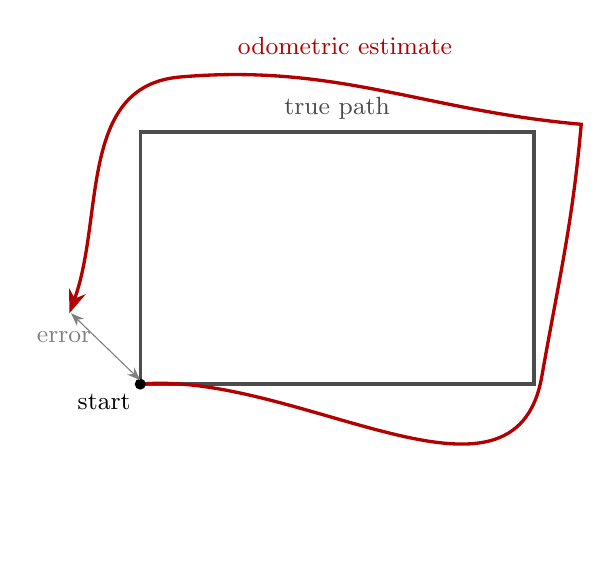
\begin{tikzpicture}[>=Stealth,every node/.style={font=\small}]
\draw[black!70,very thick] (0,0)--(5,0)--(5,3.2)--(0,3.2)--cycle;
\node[black!70] at (2.5,3.5) {true path};
\draw[red!70!black,very thick,->] (0,0) to[out=5,in=-100] (5.1,0.1) to[out=80,in=-95] (5.6,3.3) to[out=175,in=5] (0.5,3.9)
   to[out=-175,in=70] (-0.9,0.9);
\node[red!70!black] at (2.6,4.3) {odometric estimate};
\fill (0,0) circle (2pt) node[below left] {start};
\draw[<->,gray] (0,0.05)--(-0.88,0.9);
\node[gray,left] at (-0.5,0.6) {error};
\end{tikzpicture}
\caption{Conceptual sketch of odometric drift (original): the robot drives around a rectangle and returns
to its start, but the integrated estimate does not close the loop; the gap keeps growing with distance.}\label{fig:drift}
\end{figure}

\begin{figure}[H]
	\centering
	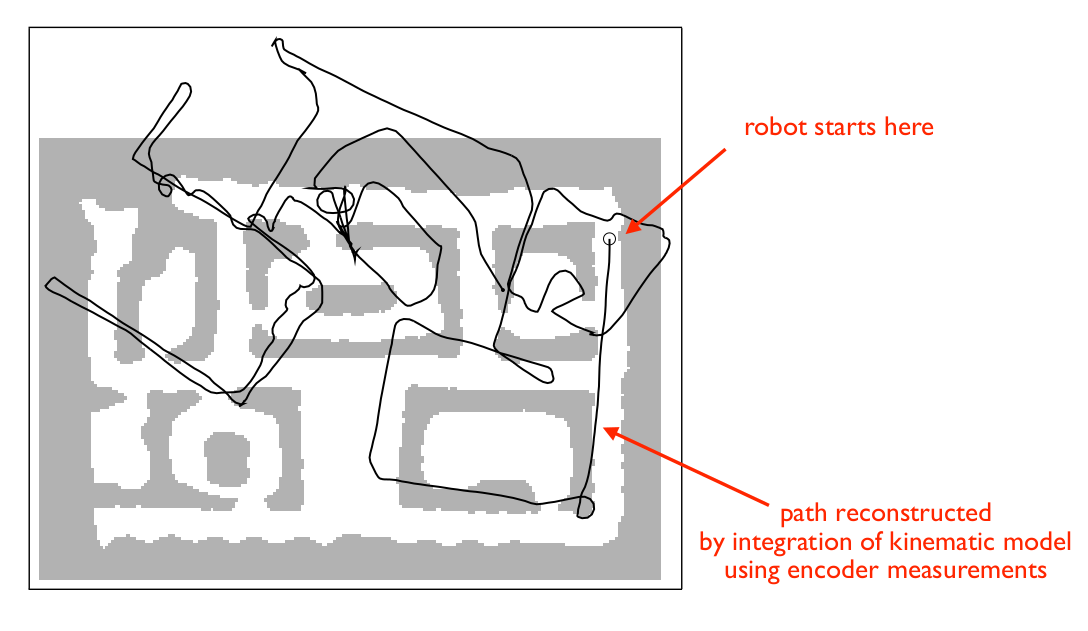
\includegraphics[width=1.0\linewidth]{1793878727480.png}
	\caption{Real experiment: path reconstructed by integrating the kinematic model with encoder measurements,
drawn over the environment map }\label{fig:1793878727480}
\end{figure}

\begin{example}[Why a $1\%$ calibration error is not small]
Differential drive with $d=0.30$ m. Suppose the true right wheel is $1\%$ larger than the nominal
radius used by the odometry, and the robot is commanded to go straight, so both encoders report the same
rotation $\Delta\phi$. The odometry concludes $\Delta\theta=0$, but physically
$\Delta\theta=\frac{0.01\,r\Delta\phi}{d}\approx\frac{0.01}{0.30}\,\Delta s\approx0.033\,\Delta s$:
the robot actually follows an arc with curvature $\approx0.033$ m$^{-1}$ (radius $\approx30$ m).
After $s=10$ m the heading is off by $\approx0.33$ rad ($\approx19^\circ$) and the lateral position by
$\approx s^2\kappa/2\approx1.7$ m, while the estimate still believes the robot is on the straight line.
\end{example}

\begin{intuition}
A tiny mismatch between the wheels is divided by the small wheelbase $d$ and becomes a heading error; a
heading error then is turned into a sideways position error that grows with the distance traveled. Errors
are never ``forgotten'' by integration --- they only add up. To stop this we need a measurement that
does not depend on the past: a landmark, a wall, a map.
\end{intuition}

% =====================================================================
\section{From dead reckoning to probabilistic localization \slides{EKF deck, slide 2}}
% =====================================================================

Dead reckoning keeps a \emph{single hypothesis} about the configuration, and its error diverges over time.
\emph{Probabilistic localization} instead maintains a probability distribution over the space of all possible
hypotheses. If a map of the environment is known, the actual readings of an exteroceptive sensor can be compared
with the readings predicted from the current estimate; the mismatch is used to reduce the odometric drift. This
idea is formalized by Bayesian estimation, and a tractable instance is the \emph{Extended Kalman Filter} (EKF).

\begin{intuition}
Walking in a dark corridor you count steps (odometry) and your belief about your position spreads out. When
your hand touches a door frame you know exists on the map, the belief suddenly shrinks. The filter
is the bookkeeping that tells you exactly how much to trust the step count versus the touch.
\end{intuition}

% =====================================================================
\section{Basic concepts: mean, covariance, Gaussians \slides{EKF deck, slides 3--4}}
% =====================================================================

\begin{definition}[Mean, covariance, multivariate Gaussian]
Let $\boldsymbol X\in\Rn^n$ be a random vector with density $f_{\boldsymbol X}(\bx)$. Its \emph{expected value} and
\emph{covariance matrix} are
\[
\bar{\boldsymbol X}=\E(\boldsymbol X)=\int_{\Rn^n}\bx\,f_{\boldsymbol X}(\bx)\,d\bx,\qquad
\mP_X=\E\big((\boldsymbol X-\bar{\boldsymbol X})(\boldsymbol X-\bar{\boldsymbol X})\tp\big).
\]
$\boldsymbol X$ is \emph{multivariate Gaussian} if
\[
f_{\boldsymbol X}(\bx)=\frac{1}{\sqrt{(2\pi)^n|\mP_X|}}\;
\exp\!\Big(-\tfrac12(\bx-\bar{\boldsymbol X})\tp\mP_X^{-1}(\bx-\bar{\boldsymbol X})\Big).
\]
\end{definition}

\begin{proposition}[Geometry of a Gaussian]\label{prop:ellipse}
The equidensity contours of a Gaussian are ellipsoids $(\bx-\bar{\boldsymbol X})\tp\mP_X^{-1}(\bx-\bar{\boldsymbol X})=c$.
Their principal axes are directed along the eigenvectors of $\mP_X$, and the squared lengths of the axes are
proportional to the corresponding eigenvalues.
\end{proposition}
\begin{proof}
Write $\mP_X=\mathbf U\boldsymbol\Lambda\mathbf U\tp$ with $\mathbf U$ orthogonal. In the coordinates
$\boldsymbol z=\mathbf U\tp(\bx-\bar{\boldsymbol X})$ the contour is $\sum_i z_i^2/\lambda_i=c$, an axis-aligned ellipsoid
with semi-axes $\sqrt{c\lambda_i}$ along the columns of $\mathbf U$.
\end{proof}

\begin{figure}[H]
\centering
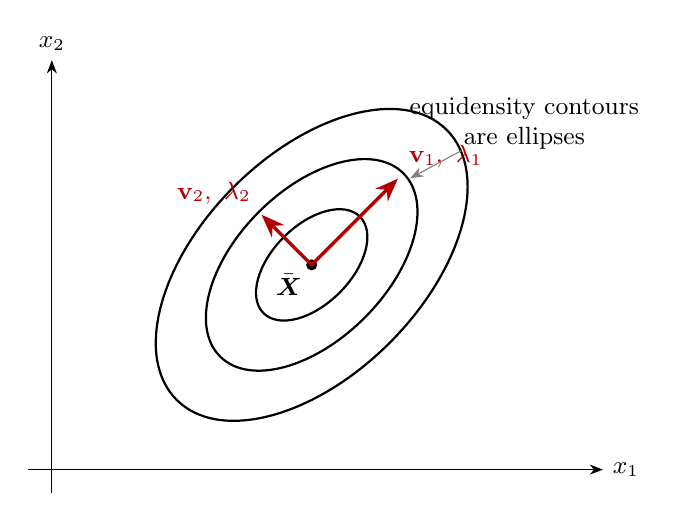
\begin{tikzpicture}[>=Stealth,every node/.style={font=\small}]
\draw[->] (-0.3,0)--(7,0) node[right] {$x_1$};
\draw[->] (0,-0.3)--(0,5.2) node[above] {$x_2$};
\def\mx{3.3}\def\my{2.6}
\foreach \k in {1,1.9,2.8}{
  \draw[rotate around={45:(\mx,\my)},thick] (\mx,\my) ellipse ({0.866*\k*1.0} and {0.5*\k*1.0});
}
\fill (\mx,\my) circle (2pt) node[below left] {$\bar{\boldsymbol X}$};
\draw[->,very thick,red!70!black] (\mx,\my)--++(45:1.55) node[above right] {$\mathbf v_1,\ \lambda_1$};
\draw[->,very thick,red!70!black] (\mx,\my)--++(135:0.9) node[above left] {$\mathbf v_2,\ \lambda_2$};
\node[align=center] at (6.0,4.4) {equidensity contours\\are ellipses};
\draw[->,gray] (5.2,4.05)--(4.55,3.7);
\end{tikzpicture}
\caption{Geometric interpretation of a covariance matrix (redrawn): ellipses centered at the mean, with axes along the
eigenvectors $\mathbf v_i$ of $\mP_X$. Drawn for $\mP_X=\begin{psmallmatrix}2&1\\1&2\end{psmallmatrix}$,
$\lambda_1=3$, $\lambda_2=1$.}\label{fig:gauss}
\end{figure}

\begin{intuition}
The covariance matrix is the ``shape of the cloud'': a long thin ellipse means ``I am quite sure in one direction and
quite unsure in the other''. Example: $\mP_X=\begin{psmallmatrix}2&1\\1&2\end{psmallmatrix}$ has
eigenvalues $3$ and $1$ with eigenvectors $(1,1)/\sqrt2$ and $(1,-1)/\sqrt2$, so the cloud is stretched along the diagonal, and
its length along that direction is $\sqrt3\approx1.7$ times the length across it. The off-diagonal term $1>0$
says that $x_1$ and $x_2$ tend to be large or small together. Filters will propagate exactly this kind of ellipse.
\end{intuition}

% =====================================================================
\section{Kalman filter without noise \slides{EKF deck, slides 5--9}}
% =====================================================================

\subsection{Recursive observer: prediction and correction}

Consider the linear discrete-time system \emph{without noise}
\begin{equation}\label{eq:lin-nonoise}
\bx_{k+1}=\mA_k\bx_k+\mB_k\bu_k,\qquad \by_k=\mC_k\bx_k .
\end{equation}
We want a \emph{recursive observer}: an estimate $\hx_{k+1}$ of $\bx_{k+1}$ computed from $\bu_k$, $\by_{k+1}$ and the previous
estimate $\hx_k$, in two steps:
\begin{enumerate}
\item \textbf{prediction}: build an intermediate estimate $\hx_{k+1|k}$ by propagating $\hx_k$ through the process dynamics,
\begin{equation}\label{eq:pred0}
\hx_{k+1|k}=\mA_k\hx_k+\mB_k\bu_k ;
\end{equation}
\item \textbf{correction (update)}: correct the prediction using the difference between the measured and the predicted output.
\end{enumerate}
Even without noise a correction is needed, because the exact initial state $\bx_0$ is unknown.

\subsection{The correction as a constrained optimization}

To be consistent with the measured output, $\bx_{k+1}$ must belong to the hyperplane
\begin{equation}\label{eq:Omega}
\Omega=\{\bx:\ \mC_{k+1}\bx=\by_{k+1}\},
\end{equation}
so the correction $\Delta\bx$ must satisfy $\mC_{k+1}(\hx_{k+1|k}+\Delta\bx)=\by_{k+1}$. There are infinitely many such
corrections; intuitively the best is the \emph{closest} to the prediction, which we believe is accurate (Fig.~\ref{fig:naive}).

\begin{proposition}[Minimum-norm correction]\label{prop:minnorm}
Assume $\mC_{k+1}$ has full row rank. The solution of
\[
\min\|\Delta\bx\|\quad\text{s.t.}\quad \mC_{k+1}\Delta\bx=\by_{k+1}-\mC_{k+1}\hx_{k+1|k}
\]
is
\begin{equation}\label{eq:dx0}
\Delta\bx=\mC_{k+1}\pinv\,\bnu_{k+1},\qquad
\mC_{k+1}\pinv=\mC_{k+1}\tp(\mC_{k+1}\mC_{k+1}\tp)^{-1},\qquad
\bnu_{k+1}=\by_{k+1}-\mC_{k+1}\hx_{k+1|k},
\end{equation}
where $\mC\pinv$ is the \emph{pseudoinverse} and $\bnu_{k+1}$ is the \emph{innovation}.
\end{proposition}
\begin{proof}
Lagrangian $\tfrac12\Delta\bx\tp\Delta\bx+\boldsymbol\lambda\tp(\bnu-\mC\Delta\bx)$. Stationarity gives
$\Delta\bx=\mC\tp\boldsymbol\lambda$; substituting in the constraint, $\bnu=\mC\mC\tp\boldsymbol\lambda$, so
$\boldsymbol\lambda=(\mC\mC\tp)^{-1}\bnu$ (invertible by full row rank) and $\Delta\bx=\mC\tp(\mC\mC\tp)^{-1}\bnu$.
\end{proof}

\begin{figure}[H]
\centering
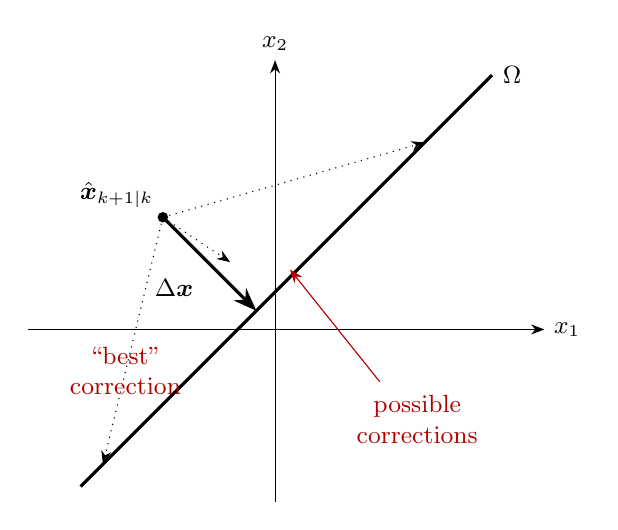
\begin{tikzpicture}[>=Stealth,every node/.style={font=\small},scale=0.95]
\draw[->] (-3.3,0)--(3.6,0) node[right] {$x_1$};
\draw[->] (0,-2.3)--(0,3.6) node[above] {$x_2$};
\draw[very thick] (-2.6,-2.1)--(2.9,3.4) node[right] {$\Omega$};
\coordinate (P) at (-1.5,1.5);
\fill (P) circle (2pt) node[above left] {$\hx_{k+1|k}$};
\draw[->,dotted] (P)--(2.0,2.5);
\draw[->,dotted] (P)--(-0.6,0.9);
\draw[->,dotted] (P)--(-2.3,-1.8);
\draw[->,very thick] (P)--(-0.25,0.25);
\node at (-1.35,0.55) {$\Delta\bx$};
\node[align=center,red!70!black] at (1.9,-1.2) {possible\\corrections};
\draw[->,red!70!black] (1.4,-0.7)--(0.2,0.8);
\node[align=center,red!70!black] at (-2.0,-0.55) {``best''\\correction};
\end{tikzpicture}
\caption{Naive correction (redrawn): among all points of the measurement hyperplane $\Omega$, pick the one closest to the
prediction; $\Delta\bx$ is orthogonal to $\Omega$.}\label{fig:naive}
\end{figure}

\begin{intuition}
The measurement tells you ``the true state is somewhere on this line''. You were already standing at the prediction, so
you take the shortest step onto the line --- a perpendicular projection. \emph{Worked numbers:} $\bx\in\Rn^2$,
$\mC=(1\ \ 1)$ (we only measure the sum $x_1+x_2$), $\hx_{k+1|k}=(1,0)$ and $y_{k+1}=3$. Then $\nu=3-1=2$,
$\mC\pinv=(\tfrac12,\tfrac12)\tp$, $\Delta\bx=(1,1)$ and $\hx_{k+1}=(2,1)$, whose sum is indeed $3$.
\end{intuition}

\subsection{Why this naive observer is not enough}

The resulting two-step observer is $\hx_{k+1|k}=\mA_k\hx_k+\mB_k\bu_k$, $\hx_{k+1}=\hx_{k+1|k}+\mC_{k+1}\pinv\bnu_{k+1}$.
In general $\hx_{k+1}$ will \emph{not} converge to $\bx_{k+1}$: the correction is naive because estimation errors
directed as $\Omega$ are not corrected. In particular the gain does not exploit the observability of the system
(unlike, e.g., a Luenberger observer).

\begin{intuition}
Take $\mA_k=\mI$, $\mC=(1\ \ 1)$, true state $(1,2)$ and $\hx_0=(0,0)$. The first correction gives
$(1.5,1.5)$, which already reproduces $y=3$, so every later innovation is zero and the error $(-0.5,\,0.5)$ never
disappears: a correction that only looks at the ``compatible with the measurement'' direction cannot fix errors along
$\Omega$. (This pair is unobservable, so no observer could do better; the point is only to see the mechanism.)
The remedy is to choose the gain in a principled way using noise statistics.
\end{intuition}

% =====================================================================
\section{Kalman filter with process noise only \slides{EKF deck, slides 10--15}}
% =====================================================================

Now include \emph{process noise}:
\begin{equation}\label{eq:lin-process}
\bx_{k+1}=\mA_k\bx_k+\mB_k\bu_k+\bv_k,\qquad \by_k=\mC_k\bx_k,
\end{equation}
where $\bv_k$ is \emph{white} (successive samples are uncorrelated), \emph{Gaussian}, zero-mean with covariance $\mV_k$.
The system is now a random process, so we compute both an estimate $\hx_{k+1}$ and its estimation-error covariance
$\mP_{k+1}$, keeping the prediction/correction structure.

\subsection{Prediction}

The state prediction is unchanged, $\hx_{k+1|k}=\mA_k\hx_k+\mB_k\bu_k$, because $\bv_k$ has zero mean.

\begin{lemma}[Covariance prediction]\label{lem:covpred}
$\mP_{k+1|k}=\mA_k\mP_k\mA_k\tp+\mV_k$.
\end{lemma}
\begin{proof}
$\bx_{k+1}-\hx_{k+1|k}=\mA_k(\bx_k-\hx_k)+\bv_k$. Expanding $\mP_{k+1|k}=\E\big((\bx_{k+1}-\hx_{k+1|k})(\cdot)\tp\big)$ gives
$\mA_k\E\big((\bx_k-\hx_k)(\bx_k-\hx_k)\tp\big)\mA_k\tp+\E(\bv_k\bv_k\tp)$ plus cross terms. By linearity of $\E$ and the independence of $\bv_k$
from $\hx_k$ and $\bx_k$ (and zero mean), the cross terms vanish. Hence $\mP_{k+1|k}=\mA_k\mP_k\mA_k\tp+\mV_k$.
\end{proof}

The predicted state distribution is Gaussian with mean $\hx_{k+1|k}$ and covariance $\mP_{k+1|k}$.

\begin{intuition}
Propagating through $\mA_k$ stretches or rotates the uncertainty ellipse; adding $\mV_k$ \emph{fattens} it: every step, the
world shakes the robot a little and we lose a bit of knowledge. With no measurements, $\mP$ can only grow --- the
covariance-level picture of odometric drift.
\end{intuition}

\subsection{State correction: Mahalanobis distance and weighted pseudoinverse}

We should choose $\Delta\bx$ so as to get the \emph{most likely} $\bx$ in $\Omega$, i.e.\ the $\bx$ that maximizes the Gaussian
$p(\bx)\propto\exp\!\big(-\tfrac12(\bx-\hx_{k+1|k})\tp\mP_{k+1|k}^{-1}(\bx-\hx_{k+1|k})\big)$. Since $p$ is maximized when the exponent is
minimized, the correction minimizes the squared \emph{Mahalanobis distance}
\begin{equation}
\|\Delta\bx\|_M^2=\Delta\bx\tp\mP_{k+1|k}^{-1}\Delta\bx ,
\end{equation}
which penalizes deviations along directions where the precision is higher.

\begin{proposition}[Weighted correction]\label{prop:weighted}
The solution of $\min\|\Delta\bx\|_M$ s.t.\ $\mC_{k+1}\Delta\bx=\by_{k+1}-\mC_{k+1}\hx_{k+1|k}$ is
\begin{equation}\label{eq:dxM}
\Delta\bx=\mC_{k+1,M}\pinv\,\bnu_{k+1},\qquad
\mC_{k+1,M}\pinv=\mP_{k+1|k}\mC_{k+1}\tp\big(\mC_{k+1}\mP_{k+1|k}\mC_{k+1}\tp\big)^{-1},
\end{equation}
the \emph{weighted pseudoinverse} of $\mC_{k+1}$.
\end{proposition}
\begin{proof}
As in Prop.~\ref{prop:minnorm} with the Lagrangian $\tfrac12\Delta\bx\tp\mP^{-1}\Delta\bx+\boldsymbol\lambda\tp(\bnu-\mC\Delta\bx)$:
stationarity gives $\Delta\bx=\mP\mC\tp\boldsymbol\lambda$, the constraint gives $\bnu=\mC\mP\mC\tp\boldsymbol\lambda$, hence
$\Delta\bx=\mP\mC\tp(\mC\mP\mC\tp)^{-1}\bnu$.
\end{proof}

\begin{figure}[H]
\centering
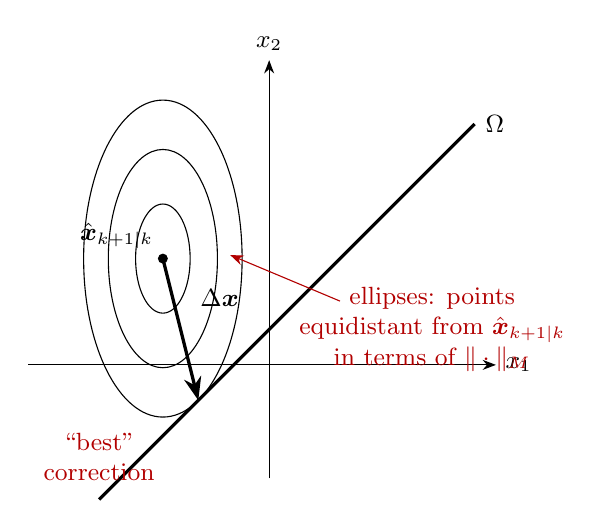
\begin{tikzpicture}[>=Stealth,every node/.style={font=\small},scale=0.9]
\draw[->] (-3.4,0)--(3.2,0) node[right] {$x_1$};
\draw[->] (0,-1.6)--(0,4.3) node[above] {$x_2$};
\draw[very thick] (-2.4,-1.9)--(2.9,3.4) node[right] {$\Omega$};
\coordinate (P) at (-1.5,1.5);
\foreach \k in {0.7,1.4,2.033}{
  \draw (P) ellipse ({0.55*\k} and {1.1*\k});
}
\fill (P) circle (2pt) node[above left] {$\hx_{k+1|k}$};
\draw[->,very thick] (P)--(-1,-0.5);
\node at (-0.7,0.95) {$\Delta\bx$};
\node[align=center,red!70!black] at (2.3,0.5) {ellipses: points\\equidistant from $\hx_{k+1|k}$\\in terms of $\|\cdot\|_M$};
\draw[->,red!70!black] (1.0,0.9)--(-0.55,1.55);
\node[align=center,red!70!black] at (-2.4,-1.3) {``best''\\correction};
\end{tikzpicture}
\caption{Weighted correction (redrawn): the best correction is the point of $\Omega$ reached by the smallest ellipse of the
current covariance estimate, i.e.\ where an ellipse is tangent to $\Omega$. Here $\mP_{k+1|k}=\diag(0.55^2,1.1^2)$, $\mC=(-1\ \ 1)$.}\label{fig:weighted}
\end{figure}

\begin{intuition}
Now ``close'' is measured with the ruler of the filter's own uncertainty: a unit of error along a well-known direction
costs a lot, along a poorly known direction it is cheap. So the filter moves mostly along the direction it is
\emph{least sure} about. \emph{Worked numbers:} same $\mC=(1\ \ 1)$, $\nu=2$ as before, but $\mP_{k+1|k}=\diag(4,1)$ ($x_1$ is more uncertain).
Then $\mC\mP\mC\tp=5$ and $\Delta\bx=\mP\mC\tp\nu/5=(1.6,\,0.4)$ instead of the isotropic $(1,1)$: the uncertain coordinate absorbs
$80\%$ of the correction.
\end{intuition}

\subsection{Covariance correction and its flaw}

\begin{proposition}[Covariance correction]\label{prop:covcorr}
With the correction \eqref{eq:dxM}, $\mP_{k+1}=\mP_{k+1|k}-\mC_{k+1,M}\pinv\mC_{k+1}\mP_{k+1|k}$.
\end{proposition}
\begin{proof}
Since $\by_{k+1}=\mC_{k+1}\bx_{k+1}$, $\bnu_{k+1}=\mC_{k+1}(\bx_{k+1}-\hx_{k+1|k})$ and the error after the correction is
$(\mI-\mC_M\pinv\mC)(\bx_{k+1}-\hx_{k+1|k})$ (indices dropped). With $\mS=\mC\mP\mC\tp$, $\mC_M\pinv=\mP\mC\tp\mS^{-1}$ and
$\mathbf X:=\mP\mC\tp\mS^{-1}\mC\mP$ (symmetric), we get
$\mP_{k+1}=(\mI-\mC_M\pinv\mC)\mP(\mI-\mC_M\pinv\mC)\tp=\mP-\mathbf X-\mathbf X+\mP\mC\tp\mS^{-1}\mS\mS^{-1}\mC\mP=\mP-\mathbf X=\mP-\mC_M\pinv\mC\mP.$
\end{proof}

The resulting two-step filter is: prediction \eqref{eq:pred0} and $\mP_{k+1|k}=\mA_k\mP_k\mA_k\tp+\mV_k$; correction
$\hx_{k+1}=\hx_{k+1|k}+\mC_{k+1,M}\pinv\bnu_{k+1}$ and $\mP_{k+1}=\mP_{k+1|k}-\mC_{k+1,M}\pinv\mC_{k+1}\mP_{k+1|k}$.

\emph{Problem:} with no measurement noise the covariance estimate becomes \emph{singular}: $\mC\mP_{k+1}=\mC\mP-\mC\mP\mC\tp\mS^{-1}\mC\mP=\mathbf 0$,
so there is no uncertainty left in the direction normal to the measurement hyperplane.

\begin{intuition}
Continue the example $\mP_{k+1|k}=\diag(4,1)$, $\mC=(1\ \ 1)$: $\mC_M\pinv\mC\mP=\tfrac15\begin{psmallmatrix}16&4\\4&1\end{psmallmatrix}$, so
$\mP_{k+1}=\begin{psmallmatrix}0.8&-0.8\\-0.8&0.8\end{psmallmatrix}$, with determinant $0$. The filter claims to know $x_1+x_2$ \emph{exactly}
(variance $0$ along $(1,1)$) --- reasonable if the sensor is perfect, but a real sensor never is. That is why we now add measurement noise.
\end{intuition}

% =====================================================================
\section{Kalman filter: the full version \slides{EKF deck, slides 16--21}}
% =====================================================================

Finally include also \emph{measurement (sensor) noise}:
\begin{equation}\label{eq:lin-full}
\bx_{k+1}=\mA_k\bx_k+\mB_k\bu_k+\bv_k,\qquad \by_k=\mC_k\bx_k+\bw_k,
\end{equation}
with $\bv_k,\bw_k$ white Gaussian, zero mean, covariances $\mV_k,\mW_k$. The dynamic equation is unchanged, so the predictions
are the same: $\hx_{k+1|k}=\mA_k\hx_k+\mB_k\bu_k$ and $\mP_{k+1|k}=\mA_k\mP_k\mA_k\tp+\mV_k$.

\subsection{State correction with a noisy measurement}

Because of the sensor noise the output is no longer certain: we only know that $\by_{k+1}$ is drawn from a Gaussian with mean
$\mC_{k+1}\bx_{k+1}$ and covariance $\mW_{k+1}$. The correction therefore proceeds as follows.
\begin{enumerate}
\item Compute the \emph{most likely output value} $\by^*_{k+1}$, given the predictions and the measured output $\by_{k+1}$.
\item Compute the associated \emph{most likely hyperplane} $\Omega^*=\{\bx:\ \mC_{k+1}\bx=\by^*_{k+1}\}$, a compromise between prediction and measurement.
\item Compute $\Delta\bx$ as before, but using $\Omega^*$ in place of $\Omega$.
\end{enumerate}

\begin{figure}[H]
\centering
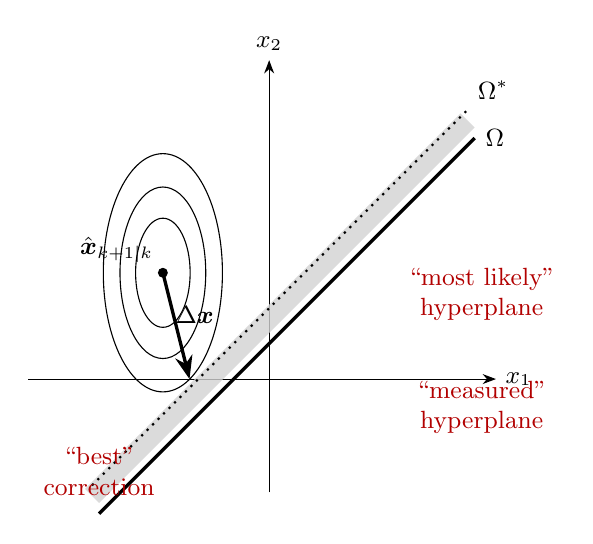
\begin{tikzpicture}[>=Stealth,every node/.style={font=\small},scale=0.9]
\draw[->] (-3.4,0)--(3.2,0) node[right] {$x_1$};
\draw[->] (0,-1.6)--(0,4.5) node[above] {$x_2$};
\fill[gray!35,opacity=0.8] (-2.6,-1.55) -- (2.7,3.75) -- (2.9,3.55) -- (-2.4,-1.75) -- cycle;
\draw[dotted,thick] (-2.5,-1.5)--(2.8,3.8) node[above right] {$\Omega^*$};
\draw[very thick] (-2.4,-1.9)--(2.9,3.4) node[right] {$\Omega$};
\coordinate (P) at (-1.5,1.5);
\foreach \k in {0.7,1.1,1.528}{
  \draw (P) ellipse ({0.55*\k} and {1.1*\k});
}
\fill (P) circle (2pt) node[above left] {$\hx_{k+1|k}$};
\draw[->,very thick] (P)--(-1.124,0);
\node at (-1.05,0.9) {$\Delta\bx$};
\node[align=center,red!70!black] at (-2.4,-1.3) {``best''\\correction};
\node[align=center,red!70!black] at (3.0,1.2) {``most likely''\\hyperplane};
\node[align=center,red!70!black] at (3.0,-0.4) {``measured''\\hyperplane};
\end{tikzpicture}
\caption{Correction with sensor noise (redrawn): the measured hyperplane $\Omega$ is uncertain (grey band); the correction targets the most
likely hyperplane $\Omega^*$, which lies between the prediction and $\Omega$. Illustrative numbers for $\mW=0.5$.}\label{fig:omegastar}
\end{figure}

\begin{theorem}[Kalman filter]\label{thm:kf}
For the system \eqref{eq:lin-full} the Kalman filter (KF) is
\begin{align}
\hx_{k+1|k}&=\mA_k\hx_k+\mB_k\bu_k,\nonumber\\
\mP_{k+1|k}&=\mA_k\mP_k\mA_k\tp+\mV_k,\nonumber\\
\hx_{k+1}&=\hx_{k+1|k}+\mR_{k+1}\bnu_{k+1},\qquad \bnu_{k+1}=\by_{k+1}-\mC_{k+1}\hx_{k+1|k},\label{eq:kf}\\
\mP_{k+1}&=\mP_{k+1|k}-\mR_{k+1}\mC_{k+1}\mP_{k+1|k},\nonumber
\end{align}
with the \emph{Kalman gain matrix}
\begin{equation}\label{eq:gain}
\mR_{k+1}=\mP_{k+1|k}\mC_{k+1}\tp\big(\mC_{k+1}\mP_{k+1|k}\mC_{k+1}\tp+\mW_{k+1}\big)^{-1}.
\end{equation}
\end{theorem}
\begin{proof}[Sketch of the gain]
Let $\mS=\mC\mP_{k+1|k}\mC\tp$ be the covariance of the predicted output. Fusing the predicted output
$\mathcal N(\mC\hx_{k+1|k},\mS)$ with the measurement (noise $\mW$) gives the most likely output
$\by^*=\mC\hx_{k+1|k}+\mS(\mS+\mW)^{-1}\bnu$. Applying Prop.~\ref{prop:weighted} with $\Omega^*$:
$\Delta\bx=\mP\mC\tp\mS^{-1}(\by^*-\mC\hx_{k+1|k})=\mP\mC\tp\mS^{-1}\mS(\mS+\mW)^{-1}\bnu=\mR_{k+1}\bnu$.
If $\mW\to0$, $\mR_{k+1}\to\mC_{k+1,M}\pinv$ and we recover the previous filter.
\end{proof}

\begin{intuition}
$\mR$ decides \emph{how much of the surprise $\bnu$ to believe}. If $\mR$ is ``large'' the measurements are more reliable than
the prediction; if $\mR$ is ``small'' the prediction is more reliable. Scalar example: $x$ with $c=1$, prior variance
$P_{k+1|k}=4$, sensor noise $W=1$. Then $R=\tfrac{4}{4+1}=0.8$. If the prediction is $0$ and the sensor reads $5$, the update is
$\hat x_{k+1}=0+0.8\cdot5=4$ (mostly the sensor), and $P_{k+1}=4-0.8\cdot4=0.8$, smaller than both $4$ and $1$: fusing two
uncertain pieces of information always yields something more certain than either. With a very noisy sensor ($W=100$) we would get
$R\approx0.04$ and the prediction would dominate.
\end{intuition}

\subsection{Properties of the KF}

\begin{itemize}
\item relatively low computational load, plus a lot of quantities can be precomputed; no measurements need to be stored;
\item it is a \emph{minimum mean-square error} (MMSE) estimator: it minimizes $\|\E(\bx_{k+1}-\hx_{k+1})\|^2$ for all $k$;
\item it is \emph{correct}: it provides mean value and covariance of the \emph{posterior} Gaussian distribution;
\item if the noises are non-Gaussian, the KF is still the best \emph{linear} estimator, but more accurate nonlinear filters may exist;
\item if the system is time-invariant and detectable, the mean-square estimation error stays bounded; it generally does not converge
to zero in the presence of persistent process noise.
\end{itemize}

\begin{figure}[H]
\centering
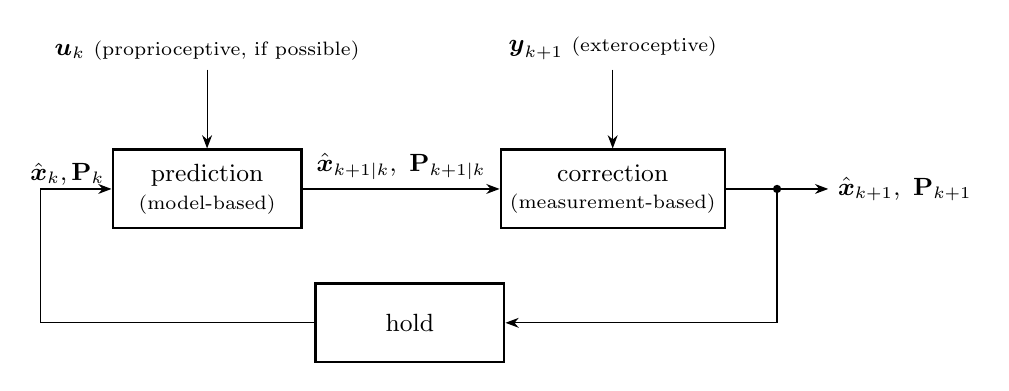
\begin{tikzpicture}[>=Stealth,every node/.style={font=\small},
  blk/.style={draw,rectangle,minimum width=2.4cm,minimum height=1.0cm,align=center,thick},
  sum/.style={draw,circle,inner sep=1pt,minimum size=0.55cm,thick}]
% top diagram
\node[blk] (pred) {prediction\\[-1pt]{\scriptsize (model-based)}};
\node[blk,right=2.5cm of pred] (corr) {correction\\[-1pt]{\scriptsize (measurement-based)}};
\node[blk] (hold) at ($(pred)!0.5!(corr)+(0,-1.7)$) {hold};
\draw[->] (pred)--(corr) node[midway,above] {$\hx_{k+1|k},\ \mP_{k+1|k}$};
\draw[->] ($(pred.north)+(0,1.0)$) node[above] {$\bu_k$\ {\scriptsize(proprioceptive, if possible)}} -- (pred.north);
\draw[->] ($(corr.north)+(0,1.0)$) node[above] {$\by_{k+1}$\ {\scriptsize(exteroceptive)}} -- (corr.north);
\draw[->] (corr.east)--++(1.3,0) coordinate (o) node[right] {$\hx_{k+1},\ \mP_{k+1}$};
\draw[->] ($(corr.east)+(0.65,0)$) |- (hold.east);
\draw[->] (hold.west) -| ($(pred.west)+(-0.9,0)$) -- (pred.west);
\node[above left,inner sep=1pt] at ($(pred.west)+(-0.05,0)$) {\small $\hx_k,\mP_k$};
\fill ($(corr.east)+(0.65,0)$) circle (1.5pt);
\end{tikzpicture}

\vspace{1.0cm}
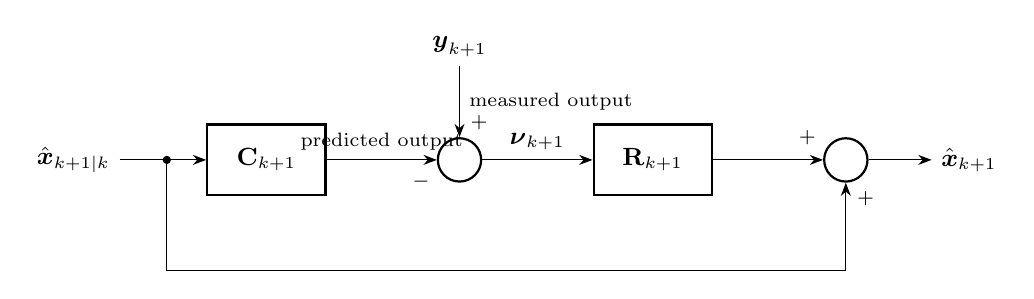
\begin{tikzpicture}[>=Stealth,every node/.style={font=\small},
  blk/.style={draw,rectangle,minimum width=1.5cm,minimum height=0.9cm,thick},
  sum/.style={draw,circle,inner sep=1pt,minimum size=0.55cm,thick}]
\node (in) {$\hx_{k+1|k}$};
\coordinate[right=0.6cm of in] (br);
\node[blk,right=0.5cm of br] (C) {$\mC_{k+1}$};
\node[sum,right=1.4cm of C] (s1) {};
\node[blk,right=1.4cm of s1] (R) {$\mR_{k+1}$};
\node[sum,right=1.4cm of R] (s2) {};
\node[right=0.8cm of s2] (out) {$\hx_{k+1}$};
\draw (in)--(br); \draw[->] (br)--(C);
\draw[->] (C)--(s1) node[midway,above] {\scriptsize predicted output};
\node[above=0.9cm of s1] (y) {$\by_{k+1}$};
\draw[->] (y)--(s1) node[midway,right] {\scriptsize measured output};
\draw[->] (s1)--(R) node[midway,above] {$\bnu_{k+1}$};
\draw[->] (R)--(s2);
\draw[->] (s2)--(out);
\fill (br) circle (1.5pt);
\draw[->] (br)--++(0,-1.4) -| (s2.south);
\node at ($(s1.west)+(-0.2,-0.28)$) {\scriptsize $-$};
\node at ($(s1.north)+(0.25,0.18)$) {\scriptsize $+$};
\node at ($(s2.west)+(-0.2,0.28)$) {\scriptsize $+$};
\node at ($(s2.south)+(0.25,-0.2)$) {\scriptsize $+$};
\end{tikzpicture}
\caption{Wrapping up (redrawn). Top: the filter alternates a model-based prediction, driven by proprioceptive data when available,
and a measurement-based correction driven by exteroceptive data; the output is held for one step and fed back. Bottom: the correction
block: the innovation $\bnu_{k+1}$ (measured minus predicted output) is weighed by the gain $\mR_{k+1}$ and added to the prediction.}\label{fig:blocks}
\end{figure}

% =====================================================================
\section{The Extended Kalman Filter \slides{EKF deck, slides 22--24}}
% =====================================================================

Consider a \emph{nonlinear} discrete-time system with noise
\begin{equation}\label{eq:nl}
\bx_{k+1}=\boldsymbol f_k(\bx_k,\bu_k)+\bv_k,\qquad \by_k=\boldsymbol h_k(\bx_k)+\bw_k,
\end{equation}
where $\boldsymbol f_k$ and $\boldsymbol h_k$ are $C^1$ functions. One simple way to build a filter: \emph{linearize} the equations
around the current estimate and apply the KF equations to the linear approximation. However, the nonlinear model is still used for
the prediction, $\hx_{k+1|k}=\boldsymbol f_k(\hx_k,\bu_k)$, and for the innovation, $\bnu_{k+1}=\by_{k+1}-\boldsymbol h_{k+1}(\hx_{k+1|k})$.

\begin{algorithm}[Extended Kalman Filter]\label{alg:ekf}
\begin{align}
\hx_{k+1|k}&=\boldsymbol f_k(\hx_k,\bu_k),\nonumber\\
\mP_{k+1|k}&=\mF_k\mP_k\mF_k\tp+\mV_k,\nonumber\\
\hx_{k+1}&=\hx_{k+1|k}+\mR_{k+1}\bnu_{k+1},\label{eq:ekf}\\
\mP_{k+1}&=\mP_{k+1|k}-\mR_{k+1}\mH_{k+1}\mP_{k+1|k},\nonumber
\end{align}
with the Jacobians and gain
\begin{gather*}
\mF_k=\frac{\partial\boldsymbol f_k}{\partial\bx}\Big|_{\bx=\hx_k},\qquad
\mH_{k+1}=\frac{\partial\boldsymbol h_{k+1}}{\partial\bx}\Big|_{\bx=\hx_{k+1|k}},\\
\mR_{k+1}=\mP_{k+1|k}\mH_{k+1}\tp\big(\mH_{k+1}\mP_{k+1|k}\mH_{k+1}\tp+\mW_{k+1}\big)^{-1}.
\end{gather*}
\end{algorithm}

Remarks. Prediction and innovation come from the nonlinear equations, while the covariance is propagated using their
\emph{linearizations}. Unlike the KF for linear-Gaussian systems, the EKF is \emph{not} guaranteed to be optimal: even with Gaussian
initial uncertainty and noises, the nonlinearity makes the state distribution non-Gaussian, and the EKF approximates it by a Gaussian.
Accuracy depends on the validity of the linearization, hence on the size of the estimation uncertainty and on the system nonlinearities.

\begin{figure}[H]
\centering
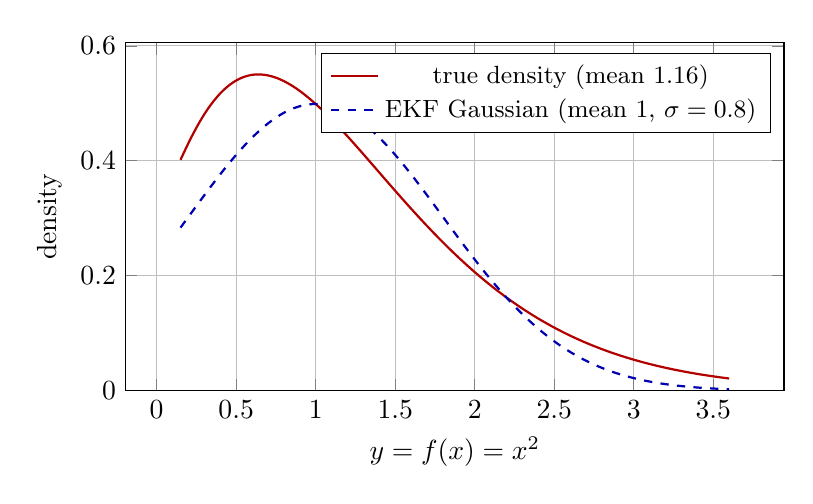
\begin{tikzpicture}
\begin{axis}[width=0.82\linewidth,height=6cm,domain=0.15:3.6,samples=200,xlabel={$y=f(x)=x^2$},
  ylabel={density},ymin=0,legend style={font=\small,at={(0.98,0.97)},anchor=north east},grid=both]
\addplot[red!70!black,thick] {1/(2*sqrt(x))*(1/(0.4*sqrt(2*pi)))*(exp(-(sqrt(x)-1)^2/(2*0.16))+exp(-(-sqrt(x)-1)^2/(2*0.16)))};
\addlegendentry{true density (mean $1.16$)}
\addplot[blue!70!black,thick,dashed] {1/(0.8*sqrt(2*pi))*exp(-(x-1)^2/(2*0.64))};
\addlegendentry{EKF Gaussian (mean $1$, $\sigma=0.8$)}
\end{axis}
\end{tikzpicture}
\caption{Why the EKF is only approximate (illustrative toy example, original): $x\sim\mathcal N(1,0.4^2)$ is passed through $f(x)=x^2$.
The true output density is skewed with mean $\mu^2+\sigma^2=1.16$; the EKF replaces it with a Gaussian centered at $f(\mu)=1$ and with
standard deviation $|f'(\mu)|\sigma=0.8$.}\label{fig:ekfapprox}
\end{figure}

\begin{intuition}
Linearizing is like replacing a curved road by its tangent line at the current estimate: fine as long as the uncertainty
cloud is small compared with the curvature, misleading when it is large. This is why an EKF that has become overconfident or has a very
large initial uncertainty can fail, and why the quality of the filter hinges on how good the estimate already is.
\end{intuition}

% =====================================================================
\section{EKF localization of a unicycle with range-and-bearing landmarks \slides{book, Sect.\ 7.7.2}}
% =====================================================================

We now apply the EKF to a unicycle equipped with a sensor that measures \emph{range} (relative distance) and \emph{bearing} to
\emph{landmarks}: easily recognizable elements of the environment, natural (features, objects) or artificial (devices added for
localization), whose positions are known to the robot. Depending on the robot configuration and the field of view, only a subset of the
landmarks is visible (Fig.~\ref{fig:landmarks}).

\begin{figure}[H]
\centering
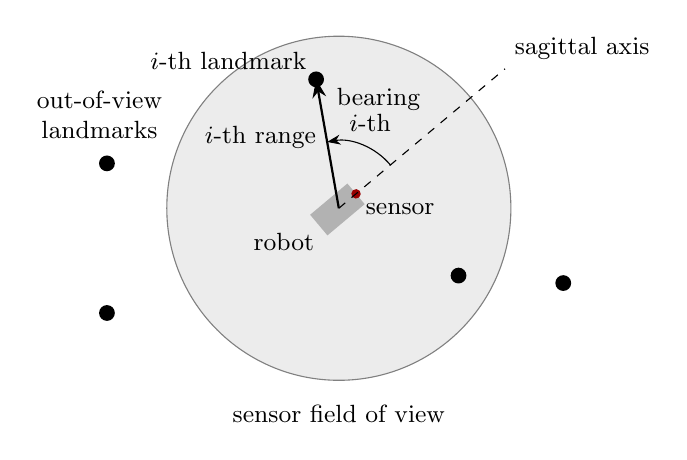
\begin{tikzpicture}[>=Stealth,every node/.style={font=\small},scale=0.95]
\fill[gray!15] (0,0) circle (2.3);
\draw[gray] (0,0) circle (2.3);
\begin{scope}[rotate around={40:(0,0)}]
  \fill[gray!60] (-0.35,-0.18) rectangle (0.3,0.18);
  \fill[red!60!black] (0.3,0) circle (1.8pt) node[below right,black] {sensor};
\end{scope}
\node[below left] at (-0.2,-0.2) {robot};
\draw[dashed] (0,0)--(40:2.9) node[above right] {sagittal axis};
\coordinate (L) at (100:1.75);
\fill (L) circle (3pt) node[above left] {$i$-th landmark};
\draw[thick,->] (0,0)--(L) node[pos=0.55,left] {$i$-th range};
\draw[->] (40:0.9) arc[start angle=40,end angle=100,radius=0.9];
\node at (70:1.22) {$i$-th};
\node at (70:1.55) {bearing};
\fill (-3.1,0.6) circle (3pt); \fill (-3.1,-1.4) circle (3pt); \fill (3.0,-1.0) circle (3pt);
\fill (1.6,-0.9) circle (3pt);
\node[align=center] at (-3.2,1.25) {out-of-view\\landmarks};
\node[align=center] at (0,-2.75) {sensor field of view};
\end{tikzpicture}
\caption{A typical setting for EKF-based localization with range and bearing measurements to known landmarks (redrawn). The bearing is measured from the
robot's sagittal axis; the landmarks outside the field of view do not produce measurements.}\label{fig:landmarks}
\end{figure}

\subsection{Motion model}

Any of the odometric models \eqref{eq:euler}, \eqref{eq:rk} or \eqref{eq:exact} can serve as the discrete-time motion model, with $v_k,\omega_k$ reconstructed from the encoders
as in Sect.~3. Taking the Euler one and adding \emph{motion noise} $\bv_k=(v_{1,k},v_{2,k},v_{3,k})$ (white, Gaussian, zero mean, covariance $\mV_k$):
\begin{equation}\label{eq:motion}
\begin{aligned}
x_{k+1}&=x_k+v_k\Ts\cos\theta_k+v_{1,k},\\
y_{k+1}&=y_k+v_k\Ts\sin\theta_k+v_{2,k},\\
\theta_{k+1}&=\theta_k+\omega_k\Ts+v_{3,k}.
\end{aligned}
\end{equation}

\subsection{Measurement model}

Let $L$ be the number of landmarks, $\boldsymbol p_{l,i}=(x_{l,i},y_{l,i})$ the known position of the $i$-th one, and $L_k$ the number of landmarks actually seen at $t_k$.
Assume the identity of each observed landmark is known (landmarks are tagged, e.g.\ by shape or color), which allows building the \emph{association map}
\[
a:\{1,\dots,L_k\}\to\{1,\dots,L\},
\]
where $a(i)$ is the identity of the $i$-th observed landmark. Assuming the sensor sits at the center of the wheel axle, the measurement model is
\begin{equation}\label{eq:meas}
\by_k=\begin{pmatrix}\boldsymbol h_1(\bq_k,a(1))\\\vdots\\\boldsymbol h_{L_k}(\bq_k,a(L_k))\end{pmatrix}+\begin{pmatrix}\bw_{1,k}\\\vdots\\\bw_{L_k,k}\end{pmatrix},\qquad
\boldsymbol h_i(\bq_k,a(i))=\begin{pmatrix}\sqrt{(x_k-x_{l,a(i)})^2+(y_k-y_{l,a(i)})^2}\\[2pt]
\atantwo(y_{l,a(i)}-y_k,\;x_{l,a(i)}-x_k)-\theta_k\end{pmatrix},
\end{equation}
with $\bw_k$ white, Gaussian, zero mean, covariance $\mW_k$. Both the motion and the measurement model are nonlinear.

\subsection{The EKF equations for this problem}

\noindent\textbf{Prediction.}
\[
\hq_{k+1|k}=\begin{pmatrix}\hat x_{k+1|k}\\\hat y_{k+1|k}\\\hat\theta_{k+1|k}\end{pmatrix}=\begin{pmatrix}\hat x_k+v_k\Ts\cos\hat\theta_k\\\hat y_k+v_k\Ts\sin\hat\theta_k\\\hat\theta_k+\omega_k\Ts\end{pmatrix},\qquad
\mP_{k+1|k}=\mF_k\mP_k\mF_k\tp+\mV_k,
\]
\begin{equation}\label{eq:F}
\mF_k=\frac{\partial\boldsymbol f}{\partial\bq_k}\Big|_{\hq_k}=\begin{pmatrix}1&0&-v_k\Ts\sin\hat\theta_k\\0&1&v_k\Ts\cos\hat\theta_k\\0&0&1\end{pmatrix}.
\end{equation}

\noindent\textbf{Correction.} $\hq_{k+1}=\hq_{k+1|k}+\mR_{k+1}\bnu_{k+1}$, $\mP_{k+1}=\mP_{k+1|k}-\mR_{k+1}\mH_{k+1}\mP_{k+1|k}$, with
$\mR_{k+1}=\mP_{k+1|k}\mH_{k+1}\tp(\mH_{k+1}\mP_{k+1|k}\mH_{k+1}\tp+\mW_{k+1})^{-1}$ and the innovation
$\bnu_{k+1}=\by_{k+1}-\boldsymbol h_{k+1}(\hq_{k+1|k})$ (actual minus predicted measurements). The matrix $\mH_{k+1}$ stacks the $L_k$ blocks
\begin{equation}\label{eq:H}
\frac{\partial\boldsymbol h_i}{\partial\bq_k}\Big|_{\hq_{k+1|k}}=
\begin{pmatrix}
\dfrac{\hat x_{k+1|k}-x_{l,a(i)}}{\rho_i} & \dfrac{\hat y_{k+1|k}-y_{l,a(i)}}{\rho_i} & 0\\[8pt]
-\dfrac{\hat y_{k+1|k}-y_{l,a(i)}}{\rho_i^2} & \dfrac{\hat x_{k+1|k}-x_{l,a(i)}}{\rho_i^2} & -1
\end{pmatrix},\qquad \rho_i=\|\boldsymbol p_{l,a(i)}-\hat{\boldsymbol p}_{k+1|k}\|,
\end{equation}
$i=1,\dots,L_k$, where $\hat{\boldsymbol p}_{k+1|k}=(\hat x_{k+1|k},\hat y_{k+1|k})$.

\begin{remark}
In the bearing row of \eqref{eq:H} the denominators are $\rho_i^2$. This follows from differentiating $\atantwo(Y,X)$, whose partial derivatives are
$-Y/(X^2+Y^2)$ and $X/(X^2+Y^2)$, with $X=x_{l}-x_k$, $Y=y_{l}-y_k$.
\end{remark}

\begin{intuition}
\emph{Reading $\mF_k$.} The third column says that a heading error $\delta\theta$ moves the predicted position sideways by
$v_k\Ts\,\delta\theta$ per step: heading uncertainty is turned into position uncertainty, and the longer the robot drives, the more
it accumulates (exactly the drift mechanism of Sect.~4, now quantified inside $\mP$).

\emph{Reading $\mH$.} The first row is the unit vector pointing from the landmark to the robot: moving the robot directly away from the landmark increases the range
at rate $1$, moving sideways does not change it (to first order). \emph{Worked numbers:} predicted pose $(0,0,0)$, landmark at $(3,4)$, so $\rho=5$:
predicted range $5$, predicted bearing $\atantwo(4,3)-0=0.927$ rad, and
$\mH_i=\begin{psmallmatrix}-0.6&-0.8&0\\0.16&-0.12&-1\end{psmallmatrix}$. Moving the robot $1$ m toward the landmark along $x$ shortens the range by about $0.6$ m
(first entry $-0.6$); a heading error of $+0.1$ rad shifts the bearing by $-0.1$ rad (last entry $-1$).
A single landmark gives two scalar equations for three unknowns $(x,y,\theta)$, so generally at least two landmarks are needed to constrain the full pose from one set of readings;
the stacked $\mH$ is what combines them.
\end{intuition}

% =====================================================================
\section{Summary}
% =====================================================================

\subsection{Comparison of methods}

\begin{table}[htbp]
\centering
\small
\renewcommand{\arraystretch}{1.25}
\begin{tabularx}{\textwidth}{@{}l>{\raggedright\arraybackslash}X>{\raggedright\arraybackslash}X>{\raggedright\arraybackslash}X@{}}
\toprule
\textbf{Integration scheme} & \textbf{Update of $x_{k+1}$ (and $y$)} & \textbf{Local error} & \textbf{Comment}\\
\midrule
Euler & $x_k+v_k\Ts\cos\theta_k$ & $\approx\tfrac12v\omega\Ts^2$ & cheapest; uses the initial heading\\
Runge--Kutta (2nd order) & $x_k+v_k\Ts\cos(\theta_k+\tfrac{\omega_k\Ts}2)$ & $\approx\tfrac1{24}v\omega^2\Ts^3$ & uses the mean heading; no division\\
Exact & $x_k+\tfrac{v_k}{\omega_k}(\sin\theta_{k+1}-\sin\theta_k)$ & none (constant inputs) & needs a conditional for $\omega_k\approx0$\\
\bottomrule
\end{tabularx}
\caption{Odometric integration schemes (all have exact $\theta_{k+1}=\theta_k+\omega_k\Ts$).}
\end{table}

\begin{table}[htbp]
\centering
\small
\renewcommand{\arraystretch}{1.25}
\begin{tabularx}{\textwidth}{@{}>{\raggedright\arraybackslash}p{2.6cm}>{\raggedright\arraybackslash}X>{\raggedright\arraybackslash}X>{\raggedright\arraybackslash}X@{}}
\toprule
\textbf{Estimator} & \textbf{Model / sensors} & \textbf{What it provides} & \textbf{Main limitation}\\
\midrule
Dead reckoning (odometry) & nonlinear kinematics; proprioceptive only & $\hq$ only; exact only if $\bq_0$, model and encoders are perfect & unbounded drift\\
Naive observer (no noise) & linear; exact output $\by$ & $\hx$ via $\mC\pinv\bnu$ (min-norm) & errors along $\Omega$ not corrected; ignores uncertainty\\
KF, process noise only & linear; exact output & $\hx,\mP$ via weighted $\mC_M\pinv$ & $\mP$ becomes singular\\
Kalman filter & linear; noisy output, Gaussian noises & $\hx,\mP$ with gain $\mR$; MMSE, correct posterior & needs linear-Gaussian setting\\
Extended Kalman filter & nonlinear $C^1$ $\boldsymbol f,\boldsymbol h$; noisy exteroceptive data (e.g.\ landmarks) & $\hx,\mP$; drift removed & approximate (linearization, Gaussian assumption); no optimality guarantee\\
\bottomrule
\end{tabularx}
\caption{From dead reckoning to the EKF.}
\end{table}

\begin{figure}[H]
\centering
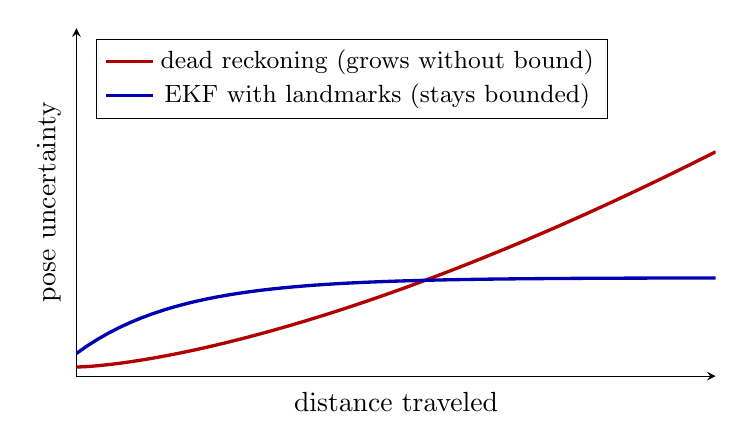
\begin{tikzpicture}
\begin{axis}[width=0.8\linewidth,height=6cm,xlabel={distance traveled},ylabel={pose uncertainty},
  xmin=0,xmax=10,ymin=0,ymax=4.6,xtick=\empty,ytick=\empty,domain=0:10,samples=60,legend pos=north west,
  legend style={font=\small},axis lines=left]
\addplot[red!70!black,very thick] {0.12+0.09*x^1.5};
\addlegendentry{dead reckoning (grows without bound)}
\addplot[blue!70!black,very thick] {0.3+1.0*(1-exp(-x/1.6))};
\addlegendentry{EKF with landmarks (stays bounded)}
\end{axis}
\end{tikzpicture}
\caption{Qualitative sketch (not measured data): pure odometry accumulates uncertainty with the distance traveled, while the EKF alternates
growth during prediction with reductions at every correction, so the uncertainty settles at a bounded level.}\label{fig:summary}
\end{figure}


\subsection{Key take-aways}

\begin{itemize}
\item \textbf{Odometry is integration.} Under piecewise-constant inputs the unicycle moves on arcs; Euler, Runge--Kutta and exact formulas differ only in how well they
follow the arc (error per step $\propto\Ts^2$, $\Ts^3$, none), and the inputs should be reconstructed from encoders ($\Delta s,\Delta\theta$), not taken from the commands.
\item \textbf{Dead reckoning always drifts.} Slippage, calibration errors and encoder noise are integrated, and small wheel errors become large heading errors
through the small wheelbase; accuracy can never be better than that of $\bq_0$.
\item \textbf{Predict, then correct.} The Kalman filter propagates a Gaussian (mean and covariance) through the model, then pulls the mean toward the measurement
along the direction the filter is least sure about, in the sense of the Mahalanobis distance.
\item \textbf{The gain $\mR=\mP\mC\tp(\mC\mP\mC\tp+\mW)^{-1}$ balances prediction and sensor.} Large $\mR$: trust the measurements; small $\mR$: trust the model. The
filter is MMSE and correct for linear-Gaussian systems.
\item \textbf{The EKF linearizes.} It keeps the nonlinear model for prediction and innovation and uses Jacobians for the covariance; this is what makes range-and-bearing
localization with known landmarks workable, at the price of approximation and no optimality guarantee.
\end{itemize}

\end{document}